\documentclass[conference]{IEEEtran}
\IEEEoverridecommandlockouts
% The preceding line is only needed to identify funding in the first footnote. If that is unneeded, please comment it out.
\usepackage{cite}
\usepackage{amsmath,amssymb,amsfonts}
\usepackage{algorithmic}
\usepackage{graphicx}
\usepackage{textcomp}
\usepackage{xcolor}
\usepackage{pgfplots}
\pgfplotsset{compat=1.17}
\def\BibTeX{{\rm B\kern-.05em{\sc i\kern-.025em b}\kern-.08em
    T\kern-.1667em\lower.7ex\hbox{E}\kern-.125emX}}
\begin{document}

\title{Angular vs Vue\\
}

\author{\IEEEauthorblockN{1\textsuperscript{st} Cornelia Langsenlehner}
\IEEEauthorblockA{\textit{Mobile Computing, BA)} \\
\textit{FH Hagenberg, Upper Austria}\\
Hagenberg, Austria\\
s2210237024@fhooe.at}
\and
\IEEEauthorblockN{2\textsuperscript{nd} Sandra Hartlauer}
\IEEEauthorblockA{\textit{Mobile Computing, BA)} \\
\textit{FH Hagenberg, Upper Austria}\\
Hagenberg, Austria\\
s2210237030@fhooe.at}
\and
\IEEEauthorblockN{3\textsuperscript{rd} Michael Nußbaumer}
\IEEEauthorblockA{\textit{Mobile Computing, BA)} \\
\textit{FH Hagenberg, Upper Austria}\\
Hagenberg, Austria\\
s2110237017@fhooe.at}
}

\maketitle

\begin{abstract}
This document is a model and instructions for \LaTeX.
This and the IEEEtran.cls file define the components of your paper [title, text, heads, etc.]. *CRITICAL: Do Not Use Symbols, Special Characters, Footnotes, 
or Math in Paper Title or Abstract.
\end{abstract}

\begin{IEEEkeywords}
component, formatting, style, styling, insert
\end{IEEEkeywords}
\section{Introduction}
\label{cha:Introduction}


\subsection{Motivation}
The increasing importance of web applications in the modern digital landscape motivates this analysis. According to the UNCTAD Digital Economy Report (2019), businesses and services are rapidly moving online, which increases the demand for efficient, user-friendly, and powerful web applications. The ability of web applications to operate across various platforms allows developers to serve a wide user base without the need to develop separate applications for each operating system or device~\cite{unctad}.

\subsection{Challenges}

%\subsection{Hardware Platforms}
Web application development necessitates compatibility across multiple hardware platforms, including desktop computers, laptops, tablets, and mobile devices. Mao (2014) identifies the primary challenge as maintaining consistent performance and efficiency across these diverse devices~\cite{mao2014developing}.

%\subsection{Frameworks}
Additionally, the selection and management of development frameworks significantly influence the efficiency and scalability of web applications. Verma (2022) points out that different frameworks exhibit unique strengths and weaknesses concerning performance, maintainability, and user-friendliness. Verma (2022) also stresses the importance of evaluation methods in assessing the performance, security, and user-friendliness of web applications. These evaluations typically include benchmarks, test scenarios, and other empirical methods aimed at verifying the quality of the application~\cite{verma2022comparison}.

\subsection{Goals}
This analysis aims to provide a brief overview of both frameworks and serve as a decision-making guide by offering valuable insights into the strengths and weaknesses of both technologies. 
These insights assist development teams in making informed decisions about the most suitable technologies for specific application requirements. Additionally, they help identify optimization opportunities to continuously enhance user experience and improve development efficiency.

\subsection{Structure}
Besides the structure, the motivation section also covers the challenges and goals of this study. The following three chapters include the theoretical background, which discusses web frameworks and compares Vue and Angular, a case study detailing a practical application and its analysis, and concludes with recommendations and future outlook.

\section{Theoretical Background}

\subsection{Web Frameworks}

Frameworks already contain numerous functions in software development as proposed solutions for individual problems faced by various developers. This way, they do not have to start from scratch whenever they want to write new software. A framework is a program skeleton that serves as a foundation for software development.

When a framework serves as the foundation for web applications, it is referred to as a web application framework. A framework describes a collection of interacting classes and thus also fixes the design structure for software developed based on the framework~\cite{ionos_webframeworks}.
\newline\subsubsection{Pros and Cons of Web Application Frameworks}
Web frameworks offer many advantages, but they also come with some disadvantages.
\subsubsection{Advantages}
\textit{Reduced Development Time and Cost:} By using templates for basic functions such as database connections, caching, and security, development time is significantly reduced.
\newline\textit{Open Source:} Most web frameworks are available as open-source, eliminating licensing costs.
\newline\textit{Clean and Maintainable Code:} Frameworks promote the creation of clean and maintainable code, as developers can rely on proven building blocks.
\newline\textit{Community Support:} Regular improvements and quick fixes for security vulnerabilities are provided by the community~\cite{ionos_webframeworks}.

\subsubsection{Disadvantages}

\textit{Framework-Specific Requirements:} Different frameworks have different design principles, potentially requiring compromises based on the project.
\newline\textit{Code Bloat:} Developers may not use all available functions, leading to unnecessary code.
\newline\textit{Dependency Risks:} Reliance on a framework and its provider can be risky if the framework is discontinued or its development slows.
\newline\textit{Learning Curve:} Familiarizing oneself with a framework’s structure and use takes time.
\newline\textit{Security Risks:} Publicly accessible source code can pose security risks for enterprise applications~\cite{ionos_webframeworks}.

\subsection{Introduction to JavaScript Web Application Frameworks and Dynamic Web Content}

JavaScript is a versatile programming language particularly suited for work in web browsers. Originally developed by Netscape, it has become one of the most widely used programming languages on the web, enabling developers to create dynamic and interactive content by manipulating the Document Object Model (DOM). Direct manipulation of the DOM can be challenging, which is where JavaScript frameworks and libraries come into play. They provide tools to simplify these and other aspects of programming, making JavaScript frameworks especially suitable for developing complex web applications. These frameworks offer a structured approach and pre-built components, enabling more efficient development once the concepts and guidelines of a particular framework are mastered~\cite{ionos_jsframeworks}.

The Document Object Model (DOM) is a programming interface for web documents. It represents the page so that programs can change the document structure, style, and content. The DOM is crucial for creating dynamic web content, which is essential for modern web applications that need to be interactive and responsive~\cite{mdn_dom}. Leveraging JavaScript frameworks and libraries facilitates the manipulation of the DOM, streamlining the creation of dynamic web content.

\subsubsection{Benefits of Dynamic Web Content}

Personalization tailors content based on user preferences, demographics, or behavior, which can significantly boost engagement and conversion rates. Personalized experiences are crucial for retaining visitors and improving user satisfaction. Real-time updates provide timely information without refreshing the entire page, which is essential for news websites, social media platforms, and e-commerce sites. JavaScript enables real-time updates through asynchronous requests and data manipulation. Enhanced user engagement through interactive features such as live chat, dynamic forms, and multimedia sliders captivates users, extending session duration and reducing bounce rates.

\subsubsection{Implementing Dynamic Web Content}

To effectively implement dynamic web content using JavaScript and jQuery, it is important to clearly define goals, whether to enhance user experience, increase conversions, or improve engagement metrics. Utilizing user data by analyzing behavior with tools like Google Analytics helps in personalizing content and tailoring dynamic elements based on preferences and interactions. Choosing appropriate technologies, such as JavaScript frameworks or libraries (e.g., React, Vue.js) and jQuery plugins, streamlines development and ensures cross-browser compatibility. Continuously testing dynamic features, gathering user feedback, and refining implementations optimize performance and user satisfaction.

jQuery is a lightweight, fast, and feature-rich JavaScript library renowned for simplifying HTML document traversal and manipulation, event handling, animation, and Ajax interactions. It provides an intuitive API that seamlessly operates across various browsers. With its versatility and extendibility, jQuery has revolutionized JavaScript development for millions of users worldwide~\cite{jquery_history}.

By leveraging JavaScript and jQuery for dynamic web content, websites can offer personalized, engaging experiences that cater to modern user expectations~\cite{moldstud2024}.

\subsection{JavaScript for Complex Web Applications}

JavaScript is well-suited for complex web applications due to its versatility and the powerful features of modern JavaScript frameworks. These frameworks provide a structured environment for development, making it easier to manage large codebases and maintain code quality.

\subsubsection{Alternatives to JavaScript}

\textit{TypeScript:} A superset of JavaScript that adds static types, making it easier to catch errors early.
\newline\textit{Dart:} Developed by Google, Dart is used in conjunction with the Flutter framework for building web and mobile apps.
\newline\textit{Elm:} A functional language that compiles to JavaScript, focused on simplicity and quality tooling~\cite{mdn-js-guide}

\subsection {Comparison Criteria}

When evaluating web development frameworks, metrics play a crucial role as they enable an objective analysis of performance and efficiency. By comparing load times, responsiveness, and resource utilization, frameworks like Angular and Vue can be assessed in various scenarios to determine their performance.

\subsubsection{Performance}
Performance metrics are measured using the developer console, focusing on loading times and responsiveness. Loading times are assessed by recording the time taken from the start of the page load until the application is fully interactive. Responsiveness is evaluated by measuring the time taken for the application to react to user inputs and interactions after the initial load, ensuring minimal delay and smooth performance.
\subsubsection{Developer-friendliness}
Angular provides a structured environment with an array of features, complemented by detailed documentation and a well-established community, as outlined in the official Angular documentation. In contrast, Vue is noted for its straightforward integration and clear syntax, which enhances ease of use and adaptability in various project sizes, according to the official Vue.js documentation~\cite{angular, vue}.

\subsubsection{Community Support}
Community support is essential for the ongoing development and troubleshooting of software frameworks. This is underscored by a study conducted by Jelica Cincović and Marija Punt, which analyzed community engagement through GitHub repository statistics. According to their findings, presented in the graph below, React commands the largest community support, with Angular and Vue also showing significant but smaller communities~\cite{cincovic2020comparison}.
% \centering
% 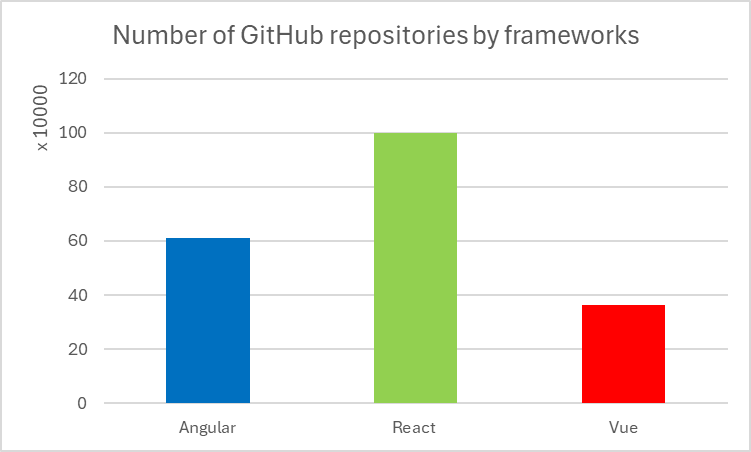
\includegraphics[width=0.6\textwidth]{image.png}
% \captionof{figure}{Number of GitHub repositories by frameworks~\cite{cincovic2020comparison}}
% \label{fig:github_repos}

\begin{figure}[h!]
    \centering
    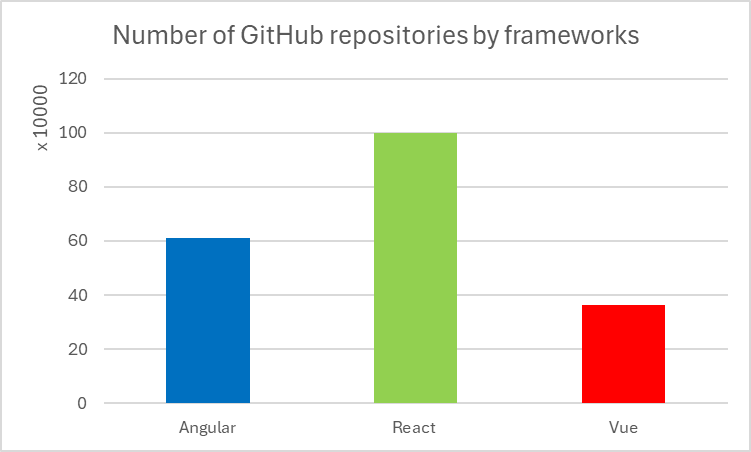
\includegraphics[width=0.5\textwidth]{image.png}
    \caption{Number of GitHub repositories by frameworks~\cite{cincovic2020comparison}}
    \label{fig:github_repos}
\end{figure}
    
% \begin{figure}[h]
% \centering
% 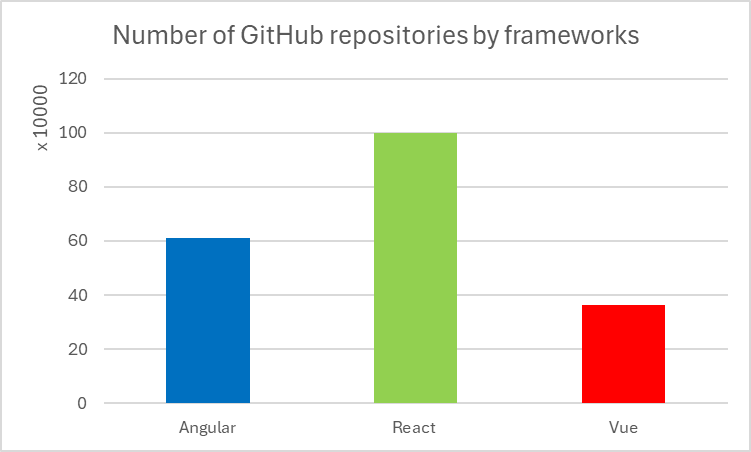
\includegraphics[width=0.6\textwidth]{image.png}
% \caption{Number of GitHub repositories by frameworks.}
% \label{fig
% }
% \end{figure}
% Active and engaged community support is crucial for framework development and bug fixing. Referring to the study by Jelica Cincović and Marija Punt titled "Comparison: Angular vs. React vs. Vue," which examined community support through GitHub repository comparisons, Figure  illustrates the following:

% \begin{figure}[h]
%     \centering
%     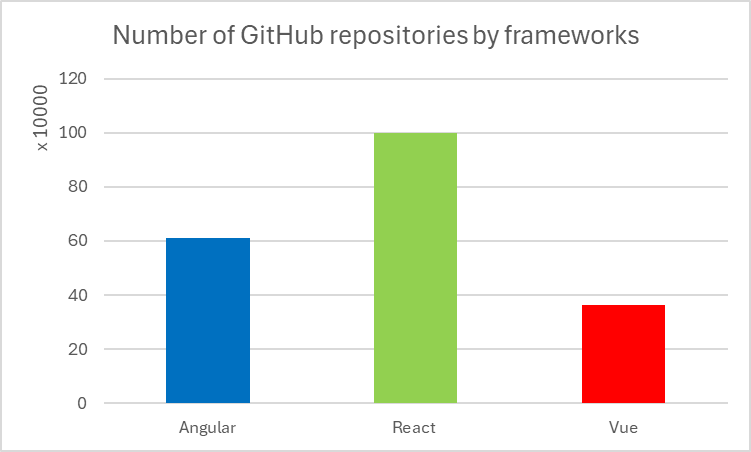
\includegraphics[width=0.6\textwidth]{image.png}
%     \caption{Number of GitHub repositories by frameworks}
%     \label{fig:github_repos}
% \end{figure}

% The graph indicates that React enjoys the largest community support, followed by Angular in second place and Vue in third~\cite{cincovic2020comparison}.
%\newpage

\subsection{Relevant JavaScript Web Application Frameworks}

Several JavaScript Web Application Frameworks are popular for developing web applications, each with its unique features and strengths. This section provides a brief overview of two of the most relevant frameworks, Vue.js and Angular, and explains why they are examined in detail.

%\section{Brief Description of Angular.js}

%AngularJS, developed by Google, is a JavaScript framework for web development that emphasizes structure and quality. It was introduced in 2010 and was the first framework suitable for large enterprise applications, emphasizing clear architecture, high testability, and isolated components. Techniques like Dependency Injection enable efficient and maintainable software development based on JavaScript.

%Angular, introduced in 2016 as a successor to AngularJS, is a complete rewrite and uses TypeScript as its foundation. This allows for better scalability and performance. Angular offers an extensive development environment with features such as two-way data binding, a powerful Command Line Interface (CLI), and a well-defined architecture. It has evolved from a pure framework to a comprehensive platform for developing web applications \cite{angular}.

%\section{Brief Description of Vue.js}

%Vue.js, pronounced /vju:/, like "view", is a JavaScript framework for designing user interfaces. It was developed by Evan You in 2014 and has quickly become one of the most popular frameworks. Vue.js is based on standard HTML, CSS, and JavaScript and offers a declarative, component-based programming model. This model allows for efficient development of user interfaces of any complexity. Key features of Vue.js include the virtual DOM, reactive data binding, and easy integration with other projects and libraries.

%Vue.js is flexible and lightweight, suitable for both small projects and large applications. It allows developers to incrementally adopt it into existing projects and add additional features as needed \cite{vuejs}.

\subsubsection{Angular}

Angular is a platform and framework for building single-page client applications using HTML and TypeScript. Developed by Google, Angular provides a comprehensive solution for complex and large-scale applications~\cite{angular-io}.
\\\\
\textit{Key Features}\\
\textit{Two-way data binding:} Angular facilitates automatic synchronization of data between model and view components.
\newline\textit{Dependency Injection:} Angular's DI system promotes modular development and testing by injecting dependencies into components.
\newline\textit{Comprehensive CLI (Command-Line Interface):} Angular CLI offers powerful tools for project scaffolding, testing, and deployment.
\newline\textit{TypeScript support:} Angular is built with TypeScript, providing type safety, enhanced tooling, and improved developer productivity.
\newline
\subsubsection{Vue}

Vue is a progressive JavaScript framework designed for building user interfaces. It is characterized by its incremental adoptability, allowing developers to integrate it gradually into existing projects without the need to fully commit to the entire framework upfront. This modular approach makes Vue suitable for both small-scale projects and large-scale applications, offering flexibility in usage based on project requirements~\cite{vuejs2024}.
\\\\
\textit{Key Features}\\
\textit{Reactive data binding:} Vue's reactive system ensures efficient updates to the DOM based on changes in data.
\newline\textit{Component-based architecture:} Vue promotes building UIs into modular, reusable components for easier maintenance and scalability.
\newline\textit{Virtual DOM:} Vue uses a virtual DOM for efficient rendering and updating of the actual DOM elements.
\newline\textit{Flexibility and integration:} Vue seamlessly integrates with existing projects and external libraries, offering flexibility in development approaches.

%\section{Differences Between Angular.js and Vue.js}

%Angular and Vue.js are both JavaScript frameworks that can be used to develop modern web applications. A key difference is that Angular uses an MVC (Model-View-Controller) architecture, while Vue.js is a more progressive framework.

%Angular provides a robust and well-established development environment with features such as efficient two-way data binding, a comprehensive CLI, and a well-defined architecture. It is particularly suitable for large and complex applications due to its strict structure and extensive tools.

%On the other hand, Vue.js is more flexible and lightweight. It uses a virtual DOM, which improves performance, and offers simple ways for CSS transitions and property computation. Vue.js is easier to learn and integrate, making it a good choice for smaller projects or projects that require rapid development.

%Both frameworks have their advantages and disadvantages, and the choice between them depends on the specific requirements and preferences of a project. While Angular offers a comprehensive solution for complex applications, Vue.js excels in simplicity and flexibility \cite{kinsta}.

\subsection{Vue vs. Angular: A Detailed Comparison}

In this section, Vue and Angular will be compoared based on several parameters to provide a clear understanding of their respective strengths and weaknesses.

\subsubsection{Performance}

\textit{Vue:} uses a virtual DOM for efficient updates and is generally faster in rendering due to its lightweight nature.
\newline\textit{Angular:} utilizes a real DOM, which can be slower in certain scenarios, and is optimized for performance with techniques like ahead-of-time (AOT) compilation.
\newline\textit{In comparison:} Vue often achieves better performance for simple to moderately complex applications. When comparing the two frameworks, Angular provides robust performance optimizations suitable for enterprise-level applications.

%\textbf{Vue:}
%\begin{itemize}
%    \item Uses a virtual DOM for efficient updates
%    \item Generally faster in rendering due to its lightweight nature
%\end{itemize}

%\textbf{Angular:}
%\begin{itemize}
%    \item Real DOM, which can be slower in certain scenarios
%    \item Optimized for performance with techniques like ahead-of-time (AOT) compilation
%\end{itemize}

%\textbf{Comparison:}
%\begin{itemize}
%    \item Vue often has better performance for simple to moderately complex applications.
%    \item Angular provides robust performance optimizations suitable for enterprise-level applications.
%\end{itemize}

\subsubsection{Developer-Friendliness}

\textit{Vue:} is easy to learn and integrate, featuring a simple syntax and flexible structure along with comprehensive documentation.
\newline\textit{Angular:} has a steeper learning curve due to its complexity and requires understanding of TypeScript, but offers extensive documentation and resources.
\newline\textit{In comparison:} Vue.js is generally more accessible for beginners, while Angular is more suitable for developers with experience in TypeScript and complex frameworks.

%\textbf{Vue:}
%\begin{itemize}
%    \item Easy to learn and integrate
%    \item Simple syntax and flexible structure
%    \item Comprehensive documentation
%\end{itemize}

%\textbf{Angular:}
%\begin{itemize}
%    \item Steeper learning curve due to its complexity
%    \item Requires understanding of TypeScript
%    \item Extensive documentation and resources
%\end{itemize}

%\textbf{Comparison:}
%\begin{itemize}
%    \item Vue.js is generally more accessible for beginners.
%    \item Angular is more suitable for developers with experience in TypeScript and complex frameworks.
%\end{itemize}

\subsection{Community Support}

\textit{Vue:} boasts a growing community with increasing adoption, complemented by numerous plugins and integrations. It benefits from active development and strong community support.
\newline\textit{Angular:} features a large and established community with extensive resources and a wide array of third-party libraries. Supported by Google, Angular ensures long-term support and robust development.
\newline\textit{In comparison:} Angular enjoys a larger and more established community base. Meanwhile, Vue is rapidly gaining traction and fostering a supportive community environment.

%\textbf{Vue:}
%\begin{itemize}
%    \item Growing community with increasing adoption
%    \item Numerous plugins and integrations
%    \item Active development and support
%\end{itemize}

%\textbf{Angular:}
%\begin{itemize}
%    \item Large and established community
%    \item Extensive resources and third-party libraries
%    \item Backed by Google, ensuring long-term support
%\end{itemize}

%\textbf{Comparison:}
%\begin{itemize}
%    \item Angular has a larger and more established community.
%    \item Vue is rapidly growing and has a supportive community.
%\end{itemize}

\subsection{Ecosystem}

\textit{Vue:} offers flexibility and seamless integration with other libraries. It provides Vue CLI for streamlined project scaffolding, along with Vue Router and Vuex for effective state management.
\newline\textit{Angular:} features a comprehensive suite of built-in tools designed for efficient development. It utilizes Angular CLI for seamless project management and includes Angular Material for building sophisticated UI components.
\newline\textit{In comparison:} Vue excels in flexibility, allowing developers to choose from a variety of tools and libraries. Meanwhile, Angular offers a more integrated and consistent development experience with its comprehensive toolset.

%\textbf{Vue:}
%\begin{itemize}
%    \item Flexible and integrates well with other libraries
%    \item Vue CLI for project scaffolding
%    \item Vue Router and Vuex for state management
%\end{itemize}

%\textbf{Angular:}
%\begin{itemize}
%    \item Comprehensive suite of built-in tools
%    \item Angular CLI for efficient development
%    \item Angular Material for UI components
%\end{itemize}

%\textbf{Comparison:}
%\begin{itemize}
%    \item Vue offers flexibility in choosing tools and libraries.
%    \item Angular provides a more integrated and consistent development experience.
%\end{itemize}

% \section{Conclusion}

% Choosing the right framework depends on the specific needs of a project. Vue.js offers simplicity and flexibility, making it ideal for smaller projects and quick integration. Angular provides a comprehensive solution suitable for large-scale applications with its robust features and strong support from Google. Understanding the strengths and weaknesses of each framework can help developers make informed decisions to best meet their project requirements.

\section{Case Study}
\label{cha:CaseStudy}

%\section{Case Study}

%In this academic paper, a detailed case study of "ProTrack," an innovative web application engineered for tracking, sharing, managing, and collaboratively editing project work is presented. ProTrack is an invaluable resource for project management and providing tools that enhance administrative efficiency.

%ProTrack has been developed in two separate versions, one using Angular.js and the other with Vue.js. This dual-framework approach allows for a comprehensive comparison, providing clear insights into the unique benefits and potential limitations that each framework offers when applied to the same functional parameters.

%The case study section delves into several critical areas of ProTrack:
%\begin{itemize}
%    \item \textbf{Functionality}: The paper thoroughly explores ProTrack's essential features, including project tracking, document sharing, task management, and collaborative capabilities. It examines how each framework supports these features and assesses their impact on the user experience.
%    \item \textbf{Development Experience}: The section offers insights from the development process with Angular.js and Vue.js, focusing on tooling support and the ease of integration with other technologies.
%    \item \textbf{Performance Metrics}: Empirical data regarding performance metrics such as load times, runtime efficiency, and resource utilization for each framework are presented. This quantitative analysis enhances the qualitative evaluations provided throughout the case study.
%\end{itemize}

%Through this examination, the case study section aims to provide a detailed assessment of both frameworks as applied to a real-world application, thereby offering essential insights that assist developers and researchers in selecting between Angular.js and Vue.js for similar projects.

%\newpage

%\subsection*{Case Study 1: Angular.js Application}

%\begin{itemize}
%    \item \textbf{Functionality}:
%    \item \textbf{Development Experience}:
%    \item \textbf{Performance Metrics}:
%\end{itemize}

%\subsection*{Case Study 2: Vue.js Application}

%\begin{itemize}
%    \item \textbf{Functionality}:
%    \item \textbf{Development Experience}:
%    \item \textbf{Performance Metrics}:
%\end{itemize}

\subsection{Introduction of the Case Study}
In this case study two versions of a web application called "ProTrack" will be compared that has been developed using two different web frameworks, Angular and Vue. ProTrack is a project management tool that allows users to track, manage and edit project work.
\subsubsection{Objective}
The objective of this case study is to compare Angular and Vue in the context of project management applications. The focus will be on three primary functionalities: user registration, project creation, and  for each project. By developing and analyzing these applications, we aim to highlight the strengths and weaknesses of each framework in practical use.
\subsubsection{Application Description}
\paragraph{User Registration and Login}
\textit{Implementation in Angular: }In Angular, user registration and login were implemented using Angular Forms and an authentication service. Angular's template-driven forms were employed to handle user input, and validation was managed through built-in validators. Authentication was handled using JSON Web Tokens (JWT) to ensure secure access.\newline
\newline\textit{Implementation in Vue: }In Vue, user registration and login were implemented using Vue Forms and Vuex for state management. The form components handled user input and validation within the components themselves. Vuex manages the user state, including authentication tokens.
\paragraph{Project Management}
\textit{Project Creation:\newline}
\textit{Angular: }Project creation in Angular was achieved using Reactive Forms and services. Reactive Forms allowed for complex form validation and dynamic form control. The data handling was managed through Angular services, ensuring a clean separation of concerns.
\newline\textit{Vue: }In Vue, project creation utilized Vue Forms and Vuex. The form logic was encapsulated within the components, while Vuex managed the state of the project data, ensuring consistency across the application.
\newline\newline
\textit{Start and Stop Functionality:\newline}
\textit{Angular: }The start and stop functionality for time tracking in Angular was implemented using a timer service and RxJS for managing time intervals. This approach allowed for reactive programming, enabling real-time updates and precise time tracking.
\newline\textit{Vue: }In Vue, the time tracking functionality was built using a timer component and Vuex for state management. The component handled the timer logic, while Vuex ensured that the state was updated accurately and consistently.
\subsection{Technical Implementation}
\paragraph{Application Architecture}
\textit{Angular: }The Angular application followed a component-based architecture with modules and services. This hierarchical structure ensured maintainability and scalability. Strong typing with TypeScript added an additional layer of robustness.
\newline\textit{Vue: }The Vue application also utilized a component-based architecture with Vuex for centralized state management. Vue's flexible structure allowed for rapid development and easy integration of new features.
\paragraph{State Management}
\textit{Angular: }State management in Angular was handled using services and BehaviorSubjects from RxJS. This approach facilitated reactive updates and a clear separation of business logic.
\newline\textit{Vue: }Vuex store was used for state management in Vue, providing a single state tree and using mutations for state changes.
\paragraph{Routing}
\textit{Angular: }The Angular Router was used for navigation, with lazy loading to improve performance. Route guards were implemented to secure routes and manage user access.
\newline\textit{Vue: }Vue Router was employed in the Vue application, with dynamic imports to optimize loading times. Navigation guards ensured that only authenticated users could access certain routes.

\subsection{Performance and Efficiency}
\subsubsection{Loading Times and Responsiveness}
\textit{Angular: }Performance metrics indicated that Angular had an up to two seconds longer initial load time due to its larger bundle size. However, once loaded, the application was highly responsive and efficient.
\newline\textit{Vue: }Vue exhibited faster initial loading times and smaller bundle sizes, contributing to a smoother user experience from the outset. Its lightweight nature made it particularly suitable for rapid development cycles.
\subsection{Challenges and Solutions}
\subsubsection{Common Challenges}
\textit{State Management and Routing:} Both frameworks encountered challenges in synchronizing state and managing navigation scenarios, such as displaying the specific data content of a particular project. Angular leveraged RxJS, while Vue utilized Vuex, both providing robust solutions to these issues.
\subsubsection{Framework-Specific Challenges}
\textit{Angular: }The main challenge with Angular was its complexity and boilerplate code, which required a steeper learning curve and more initial setup time.
\newline\textit{Vue: }Vue's flexibility sometimes led to inconsistencies. Ensuring code quality and maintaining state consistency were key challenges.

\subsection{Comparison and Analysis}
\subsubsection{Advantages and Disadvantages}
\textit{Angular: }Angular's strengths lie in its stability and comprehensive ecosystem, making it ideal for large-scale enterprise applications. However, its verbose syntax and higher initial complexity can be drawbacks.
\newline\textit{Vue: }Vue's simplicity and flexibility make it suitable for rapid development and smaller projects. Its main weakness is a less extensive ecosystem compared to Angular.

\section{Conclusion and Recommendations}
Choosing the right framework depends largely on the specific needs of a project. Vue.js offers simplicity and flexibility, making it ideal for smaller projects and rapid integration, while Angular provides a comprehensive solution suitable for large-scale applications with its robust features and strong support from Google. Understanding the strengths and weaknesses of each framework can help developers make informed decisions to best meet their project requirements.

\subsection{Summary}
Angular and Vue are tailored for different project scales and requirements. Angular is well-suited for large-scale, complex applications, benefiting from its comprehensive features and strong backing by Google. On the other hand, Vue is perfect for smaller, agile projects that require quick setups and less rigid structural constraints.

\subsection{Recommendations}
For enterprise-level applications that demand robust architecture and extensive features, Angular is the recommended choice. For projects that prioritize rapid prototyping and require a high degree of flexibility, Vue is more appropriate.

\subsection{Future Outlook}
Future research should focus on the evolving best practices in using these frameworks and how they affect development efficiency and performance. This could provide deeper insights into which frameworks are best suited for various types of projects as technology and market demands continue to evolve.

\section*{References}

Please number citations consecutively within brackets \cite{b1}. The 
sentence punctuation follows the bracket \cite{b2}. Refer simply to the reference 
number, as in \cite{b3}---do not use ``Ref. \cite{b3}'' or ``reference \cite{b3}'' except at 
the beginning of a sentence: ``Reference \cite{b3} was the first $\ldots$''

Number footnotes separately in superscripts. Place the actual footnote at 
the bottom of the column in which it was cited. Do not put footnotes in the 
abstract or reference list. Use letters for table footnotes.

Unless there are six authors or more give all authors' names; do not use 
``et al.''. Papers that have not been published, even if they have been 
submitted for publication, should be cited as ``unpublished'' \cite{b4}. Papers 
that have been accepted for publication should be cited as ``in press'' \cite{b5}. 
Capitalize only the first word in a paper title, except for proper nouns and 
element symbols.

For papers published in translation journals, please give the English 
citation first, followed by the original foreign-language citation \cite{b6}.

\begin{thebibliography}{00}
\bibitem{b1} G. Eason, B. Noble, and I. N. Sneddon, ``On certain integrals of Lipschitz-Hankel type involving products of Bessel functions,'' Phil. Trans. Roy. Soc. London, vol. A247, pp. 529--551, April 1955.
\bibitem{b2} J. Clerk Maxwell, A Treatise on Electricity and Magnetism, 3rd ed., vol. 2. Oxford: Clarendon, 1892, pp.68--73.
\bibitem{b3} I. S. Jacobs and C. P. Bean, ``Fine particles, thin films and exchange anisotropy,'' in Magnetism, vol. III, G. T. Rado and H. Suhl, Eds. New York: Academic, 1963, pp. 271--350.
\bibitem{b4} K. Elissa, ``Title of paper if known,'' unpublished.
\bibitem{b5} R. Nicole, ``Title of paper with only first word capitalized,'' J. Name Stand. Abbrev., in press.
\bibitem{b6} Y. Yorozu, M. Hirano, K. Oka, and Y. Tagawa, ``Electron spectroscopy studies on magneto-optical media and plastic substrate interface,'' IEEE Transl. J. Magn. Japan, vol. 2, pp. 740--741, August 1987 [Digests 9th Annual Conf. Magnetics Japan, p. 301, 1982].
\bibitem{b7} M. Young, The Technical Writer's Handbook. Mill Valley, CA: University Science, 1989.
\end{thebibliography}
\vspace{12pt}
\color{red}
IEEE conference templates contain guidance text for composing and formatting conference papers. Please ensure that all template text is removed from your conference paper prior to submission to the conference. Failure to remove the template text from your paper may result in your paper not being published.

\end{document}
